
\documentclass[notes,serif]{beamer}
\usepackage{graphicx}
\usepackage{url}
\usepackage{clrscode}
\usepackage{amssymb,amsmath}

% You should run 'pdflatex' TWICE, because of TOC issues.

\mode<presentation>
{
  % A tip: pick a theme you like first, and THEN modify the color theme, and then add math content.
  % Warsaw is the theme selected by default in Beamer's installation sample files.

  %%%%%%%%%%%%%%%%%%%%%%%%%%%% THEME
  %\usetheme{AnnArbor}
  %\usetheme{Antibes}
  %\usetheme{Bergen}
  %\usetheme{Berkeley}
  %\usetheme{Berlin}
  %\usetheme{Boadilla}
  %\usetheme{boxes}
  %\usetheme{CambridgeUS}
  %\usetheme{Copenhagen}
  %\usetheme{Darmstadt}
  %\usetheme{default}
  %\usetheme{Dresden}
  %\usetheme{Frankfurt}
  %\usetheme{Goettingen}
  %\usetheme{Hannover}
  %\usetheme{Ilmenau}
  %\usetheme{JuanLesPins}
  %\usetheme{Luebeck}
  %\usetheme{Madrid}
  %\usetheme{Malmoe}
  %\usetheme{Marburg}
  %\usetheme{Montpellier}
  %\usetheme{PaloAlto}
  %\usetheme{Pittsburgh}
  %\usetheme{Rochester}
  %\usetheme{Singapore}
  %\usetheme{Szeged}
  \usetheme{Warsaw}

  %%%%%%%%%%%%%%%%%%%%%%%%%%%% COLOR THEME
  %\usecolortheme{albatross}
  %\usecolortheme{beetle}
  %\usecolortheme{crane}
  \usecolortheme{default}
  %\usecolortheme{dolphin}
  %\usecolortheme{dove}
  %\usecolortheme{fly}
  %\usecolortheme{lily}
  %\usecolortheme{orchid}
  %\usecolortheme{rose}
  %\usecolortheme{seagull}
  %\usecolortheme{seahorse}
  %\usecolortheme{sidebartab}
  %\usecolortheme{structure}
  %\usecolortheme{whale}

  %%%%%%%%%%%%%%%%%%%%%%%%%%%% OUTER THEME
  %\useoutertheme{default}
  %\useoutertheme{infolines}
  %\useoutertheme{miniframes}
  %\useoutertheme{shadow}
  %\useoutertheme{sidebar}
  %\useoutertheme{smoothbars}
  %\useoutertheme{smoothtree}
  %\useoutertheme{split}
  %\useoutertheme{tree}

  %%%%%%%%%%%%%%%%%%%%%%%%%%%% INNER THEME
  %\useinnertheme{circles}
  %\useinnertheme{default}
  %\useinnertheme{inmargin}
  %\useinnertheme{rectangles}
  %\useinnertheme{rounded}

  %%%%%%%%%%%%%%%%%%%%%%%%%%%%%%%%%%%

%  \setbeamercovered{transparent} % or whatever (possibly just delete it)
  \setbeamercovered{invisible} % or whatever (possibly just delete it)
  % To change behavior of \uncover from graying out to totally invisible, can change \setbeamercovered to invisible instead of transparent. apparently there are also 'dynamic' modes that make the amount of graying depend on how long it'll take until the thing is uncovered.

}


% Get rid of nav bar
\beamertemplatenavigationsymbolsempty

% Use short top
%\usepackage[headheight=12pt,footheight=12pt]{beamerthemeboxes}
%\addheadboxtemplate{\color{black}}{
%\hskip0.3cm
%\color{white}
%\insertshortauthor \ \ \ \
%\insertframenumber \ \ \ \ \ \ \
%\insertsection \ \ \ \ \ \ \ \ \ \ \ \ \ \ \ \ \  \insertsubsection
%\hskip0.3cm}
%\addheadboxtemplate{\color{black}}{
%\color{white}
%\ \ \ \
%\insertsection
%}
%\addheadboxtemplate{\color{black}}{
%\color{white}
%\ \ \ \
%\insertsubsection
%}

% Insert frame number at bottom of the page.
\usefoottemplate{\hfil\tiny{\color{black!90}\insertframenumber}}

\usepackage[english]{babel}
\usepackage[latin1]{inputenc}

\usepackage{times}
\usepackage[T1]{fontenc}

\title{Network Programming}
\subtitle{Lecture 4---Elementary Sockets III: \\Socket Options, UDP Sockets, Name and Address Conversions}

\author{Lei Wang\\ lei.wang@dlut.edu.cn}

\institute{Dalian University of Technology}

%\date{Date}
\date{Dec 8, 2008}

\subject{Talks}

\def\defn#1{{\color{red} #1}}

\begin{document}

\begin{frame}
  \titlepage
\end{frame}

\begin{frame}
  \frametitle{Part 2. Elementary Sockets III: \\Socket Options, Name and Address Conversions}
  \tableofcontents
\end{frame}

\section{Socket Options: \texttt{getsockopt} and \texttt{setsockopt} function}
\subsection{Introduction}
\begin{frame}
\frametitle{Introduction}

There are three ways to get and set the options that affect a socket:
\begin{itemize}
  \item The \texttt{getsockopt} and \texttt{setsockopt} functions
  \item The \texttt{fcntl} function
  \item The \texttt{ioctl} function (chapter 17)
\end{itemize}
\end{frame}

\subsection{\texttt{getsockopt} and \texttt{setsockopt} Functions}

\begin{frame}[containsverbatim]
\frametitle{\texttt{getsockopt} and \texttt{setsockopt} Functions}
{\scriptsize
  \begin{verbatim}
#include <sys/socket.h>

int getsockopt(int sockfd, int level, int optname,
               void *optval, socklen_t *optlen);

int setsockopt(int sockfd, int level, int optname,
               const void *optval socklen_t optlen);
  \end{verbatim}
  \begin{flushright}
  Both return: 0 if OK, -1 on error
  \end{flushright}

}
\end{frame}

\begin{frame}
\frametitle{Summary of Socket Options}
You may refer back to them later---not required at this time.
  \begin{itemize}
    \item Figure 7.1
    \item Figure 7.2
  \end{itemize}
\end{frame}

\subsection{\texttt{checkopts.c}}
\begin{frame}
\frametitle{\texttt{checkopts.c}---experiment assignment}
  \texttt{sockopt/checkopts.c}
\end{frame}

\subsection{\texttt{fcntl} Function}
\begin{frame}
\frametitle{\texttt{fcntl} Function}
  \texttt{fcntl}: stands for "file control" and performs various descriptor control operations.
  \begin{center}
  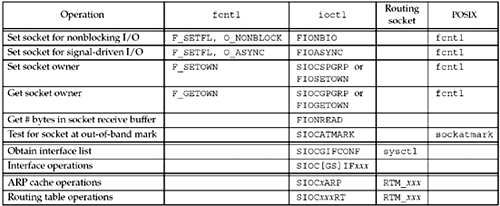
\includegraphics[width=.9\textwidth]{figs/07fig20.png}
  \end{center}
\end{frame}

\section{UDP Sockets Introduciton}
\subsection{UDP Sockets Introduciton}
\begin{frame}
\frametitle{UDP Sockets Introduciton}
  \begin{center}
  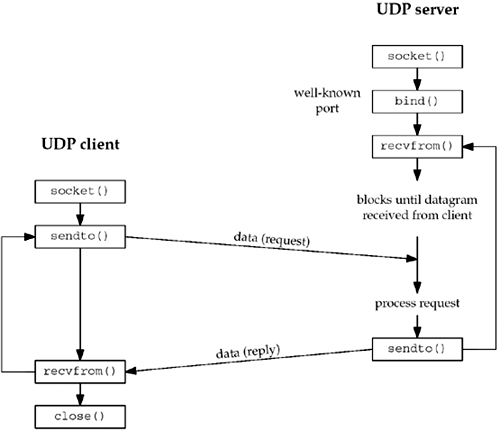
\includegraphics[width=.7\textwidth]{figs/08fig01.png}
  \end{center}
\end{frame}

\subsection{\texttt{recvfrom} and \texttt{sendto} Functions}
\begin{frame}[containsverbatim]
\frametitle{\texttt{recvfrom} and \texttt{sendto} Functions}
{\scriptsize
  \begin{verbatim}
#include <sys/socket.h>

ssize_t recvfrom(int sockfd, void *buff, size_t nbytes, 
                 int flags, struct sockaddr *from, 
                 socklen_t *addrlen);

ssize_t sendto(int sockfd, const void *buff, size_t nbytes, 
               int flags, const struct sockaddr *to, 
               socklen_t addrlen);
  \end{verbatim}
  \begin{flushright}
  Both return: number of bytes read or written if OK, �C1 on error
  \end{flushright}
}
\end{frame}

\subsection{A UDP Example}
\begin{frame}
\frametitle{UDP Echo Example: UDP Echo Server}
  \begin{center}
  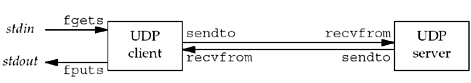
\includegraphics[width=.9\textwidth]{figs/08fig02.png}
  \end{center}
\end{frame}

\begin{frame}
\frametitle{UDP Echo Example: TCP example revisited (2 clients)}
  \begin{center}
  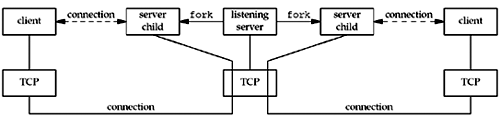
\includegraphics[width=1.0\textwidth]{figs/08fig05.png}
  \end{center}
\end{frame}

\begin{frame}
\frametitle{UDP Echo Example: UDP (2 clients)}
  \begin{center}
  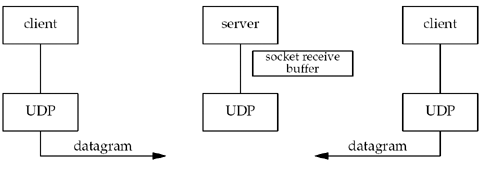
\includegraphics[width=1.0\textwidth]{figs/08fig06.png}
  \end{center}
\end{frame}

\begin{frame}
\frametitle{UDP Echo Example: Summary (from client's perspective)}
  \begin{center}
  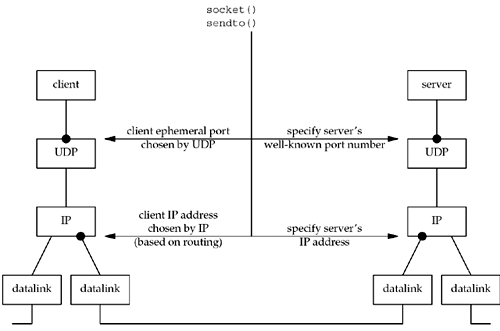
\includegraphics[width=.9\textwidth]{figs/08fig11.png}
  \end{center}
\end{frame}

\begin{frame}
\frametitle{UDP Echo Example: Summary (from server's perspective)}
  \begin{center}
  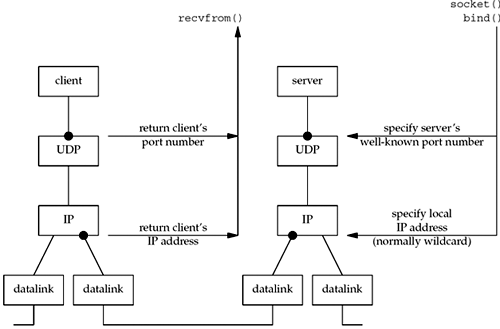
\includegraphics[width=.9\textwidth]{figs/08fig12.png}
  \end{center}
\end{frame}

\section{Name and Address Conversions}
\begin{frame}
\frametitle{Name and Address Conversions}
\begin{itemize}
  \item Domain Name System (DNS)
  \item \texttt{gethostbyname} and \texttt{gethostbyaddr} Functions
  \item \texttt{getservbyname} and \texttt{getservbyport} Functions
  \item \texttt{getaddrinfo} Function
\end{itemize}
\end{frame}

\subsection{DNS}
\begin{frame}
\frametitle{Resolvers and Name Servers}
  \begin{center}
  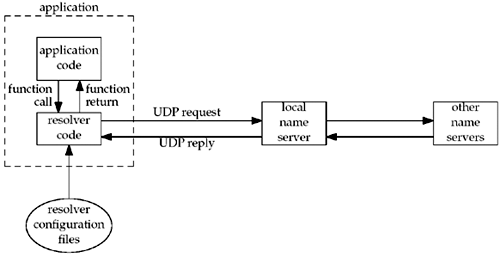
\includegraphics[width=.9\textwidth]{figs/11fig01.png}
  \end{center}
\end{frame}

\subsection{\texttt{gethostbyname} and \texttt{gethostbyaddr} Functions}
\begin{frame}[containsverbatim]
\frametitle{\texttt{gethostbyname} Function}
{\scriptsize
  \begin{verbatim}
#include <netdb.h>

struct hostent *gethostbyname (const char *hostname);
  \end{verbatim}
  \begin{flushright}
  Returns: non-null pointer if OK, \texttt{NULL} on error with \texttt{h\_errno} set
  \end{flushright}
}

{\scriptsize
  \begin{verbatim}
struct hostent {
  char  *h_name;      /* official (canonical) name of host */
  char **h_aliases;   /* pointer to array of pointers to alias names*/
  int    h_addrtype;  /* host address type: AF_INET */
  int    h_length;    /* length of address: 4 */
  char **h_addr_list; /* ptr to array of ptrs with IPv4 addrs */
};
  \end{verbatim}
}

\textbf{Example:} \texttt{names/hostent.c}
\end{frame}

\begin{frame}[containsverbatim]
\frametitle{\texttt{gethostbyaddr} Function}
{\scriptsize
  \begin{verbatim}
#include <netdb.h>

struct hostent *gethostbyaddr (const char *addr, socklen_t len, int family);
  \end{verbatim}
  \begin{flushright}
  Returns: non-null pointer if OK, \texttt{NULL} on error with \texttt{h\_errno} set
  \end{flushright}
}

\textbf{Example:} \texttt{names/hostent.c}
\end{frame}

\subsection{\texttt{getservbyname} and \texttt{getservbyport} Function}
\begin{frame}[containsverbatim]
\frametitle{\texttt{getservbyname} Function}
{\scriptsize
  \begin{verbatim}
#include <netdb.h>

struct servent *
    getservbyname (const char *servname, const char *protoname);
  \end{verbatim}
  \begin{flushright}
  Returns: non-null pointer if OK, \texttt{NULL} on error
  \end{flushright}
}

{\scriptsize
  \begin{verbatim}
struct servent {
  char   *s_name;      /* official service name */
  char  **s_aliases;   /* alias list */
  int     s-port;      /* port number, network-byte order */
  char   *s_proto;     /* protocol to use */
};
  \end{verbatim}
}
  \begin{flushleft}
  \textbf{Examples:}
  \end{flushleft}
 
{\scriptsize
  \begin{verbatim} 
struct servent *sptr;

sptr = getservbyname("domain", "udp"); /* DNS using UDP */
sptr = getservbyname("ftp", NULL);     /* FTP using TCP */
sptr = getservbyname("ftp", "udp");    /* this call will fail */
  \end{verbatim}
}

\end{frame}

\subsection{\texttt{getaddrinfo} Function}
\begin{frame}[containsverbatim]
\frametitle{\texttt{getaddrinfo} Function}
{\scriptsize
  \begin{verbatim}
#include <netdb.h>

int getaddrinfo (const char *hostname, const char *service, 
                 const struct addrinfo *hints, 
                 struct addrinfo **result) ;
  \end{verbatim}
  \begin{flushright}
  Returns: 0 if OK, nonzero on error (see Figure 11.7)
  \end{flushright}
}

{\tiny
  \begin{verbatim}
struct addrinfo {
   int          ai_flags;           /* AI_PASSIVE, AI_CANONNAME */
   int          ai_family;          /* AF_xxx */
   int          ai_socktype;        /* SOCK_xxx */
   int          ai_protocol;        /* 0 or IPPROTO_xxx for IPv4 and IPv6 */
   socklen_t    ai_addrlen;         /* length of ai_addr */
   char        *ai_canonname;       /* ptr to canonical name for host */
   struct sockaddr    *ai_addr;     /* ptr to socket address structure */
   struct addrinfo    *ai_next;     /* ptr to next structure in linked list */
};
  \end{verbatim}
}

\end{frame}

%\begin{frame}
%\frametitle{...}
%\begin{itemize}
%  \item
%  \item
%  \item
%  \item
%  \item
%\end{itemize}
%\end{frame}

%%
%\begin{frame}
%\frametitle{...}
%\begin{itemize}
%  \item
%  \item
%  \item
%  \item
%  \item
%\end{itemize}
%\end{frame}

\end{document}
